\newcommand{\svcourse}{CST Part IA: Introduction to Probability}
\newcommand{\svnumber}{1}
\newcommand{\svvenue}{Churchill, Room TBD}
\newcommand{\svdate}{2022-05-14}
\newcommand{\svtime}{11:00}
\newcommand{\svuploadkey}{PO5ogKIM8KQA22FZS8IAf8gxA8XKi19jxIBVHIfFZ+3GCBXuNUXS9lVN6bNYjxM/}

\newcommand{\svrname}{Mr Matthew Ireland}
\newcommand{\jkfside}{twoside}
\newcommand{\jkfhanded}{right}

\newcommand{\studentname}{Harry Langford}
\newcommand{\studentemail}{hjel2@cam.ac.uk}


\documentclass[10pt,\jkfside,a4paper]{article}

\input{../../template/includes.tex}
% DO NOT add \usepackage commands here.  Place any custom commands
% into your SV work files.  Anything in the template directory is
% likely to be overwritten!

\usepackage{fancyhdr}

\usepackage{lastpage}       % ``n of m'' page numbering
\usepackage{lscape}         % Makes landscape easier

\usepackage{verbatim}       % Verbatim blocks
\usepackage{epsfig}         % Embed encapsulated postscript
\usepackage{array}          % Array environment
\usepackage[nolinks]{qrcode}         % QR codes
\usepackage{enumitem}       % Required by Tom Johnson's exam question header

\usepackage{hhline}         % Horizontal lines in tables
\usepackage{siunitx}        % Correct spacing of units
\usepackage{amsmath}        % American Mathematical Society
\usepackage{amssymb}        % Maths symbols
\usepackage{amsthm}         % Theorems

\usepackage{ifthen}         % Conditional processing in tex

\usepackage[top=3cm,
            bottom=3cm,
            inner=2cm,
            outer=5cm]{geometry}

% PDF metadata + URL formatting
\usepackage[
            pdfauthor={\studentname},
            pdftitle={\svcourse, SV \svnumber},
            pdfsubject={},
            pdfkeywords={9d2547b00aba40b58fa0378774f72ee6},
            pdfproducer={},
            pdfcreator={},
            hidelinks]{hyperref}

\renewcommand{\headrulewidth}{0.4pt}
\renewcommand{\footrulewidth}{0.4pt}
\fancyheadoffset[LO,LE,RO,RE]{0pt}
\fancyfootoffset[LO,LE,RO,RE]{0pt}
\pagestyle{fancy}
\fancyhead{}
\fancyhead[LO,RE]{{\bfseries \studentname}\\\studentemail}
\fancyhead[RO,LE]{{\bfseries \svcourse, SV~\svnumber}\\\svdate\ \svtime, \svvenue}
\fancyfoot{}
\fancyfoot[LO,RE]{For: \svrname}
\fancyfoot[RO,LE]{\today\hspace{1cm}\thepage\ / \pageref{LastPage}}
\fancyfoot[C]{\qrcode[height=0.8cm]{\svuploadkey}}
\setlength{\headheight}{22.55pt}

\ifthenelse{\equal{\jkfside}{oneside}}{

 \ifthenelse{\equal{\jkfhanded}{left}}{
  % 1. Left-handed marker, one-sided printing or e-marking, use oneside and...
  \evensidemargin=\oddsidemargin
  \oddsidemargin=73pt
  \setlength{\marginparwidth}{111pt}
  \setlength{\marginparsep}{-\marginparsep}
  \addtolength{\marginparsep}{-\textwidth}
  \addtolength{\marginparsep}{-\marginparwidth}
 }{
  % 2. Right-handed marker, one-sided printing or e-marking, use oneside.
  \setlength{\marginparwidth}{111pt}
 }

}{
 % 3. Alternating margins, two-sided printing, use twoside.
}

\setlength{\parindent}{0em}
\addtolength{\parskip}{1ex}

% Exam question headings, labels and sensible layout (courtesy of Tom Johnson)
\setlist{parsep=\parskip, listparindent=\parindent}
\newcommand{\examhead}[3]{\section{#1 Paper #2 Question #3}}
\newenvironment{examquestion}[3]{
    \examhead{#1}{#2}{#3}\setlist[enumerate, 1]{label=(\alph*)}\setlist[enumerate, 2]{label=(\roman*)}
    \marginpar{\qrcode{https://www.cl.cam.ac.uk/teaching/exams/pastpapers/y#1p#2q#3.pdf}}
    \marginpar{\footnotesize \url{https://www.cl.cam.ac.uk/teaching/exams/pastpapers/y#1p#2q#3.pdf}}
}{}



\usepackage{enumitem}
\usepackage{listings}
\usepackage{tikz}

\begin{document}

\begin{examquestion}{2009}{1}{6}

\begin{enumerate}[label=(\alph*)]

\item State the defining properties of a min-heap. Show how to convert between the
tree and the (zero-based) array representation of a min-heap.

Every element in a min heap is smaller than both its children.

There are two possibilities when converting between the tree-based and array-based representation 
of the heap:

\begin{itemize}

\item The tree is almost-full

\item The tree is not almost-full

\end{itemize}

In the first case where the tree is almost-full, all we must do is a breadth-first traversal 
of the tree and store the output into an array.

However, if the tree is not almost-full then conversion to a heap-based representation is more 
complicated. All we can do is place the elements in the tree into an array and then heapify the 
array.

So we do traverse the tree and place every node we encounter into an array (either
a pre-order dfs for minimum space complexity or a breadth-first search to preserve as much ordering 
as possible and minimise the number of swaps we have to do when calling heapify). 
Now we have an array containing the elements of the tree. This has taken $\Theta(n)$ time.

We now apply the algorithm to turn an unsorted array into a heap. This involves recursively 
``merging'' heaps inside the array and adding another element at the same time. Initially these 
heaps are the leaf nodes and one parent. However as the parents become the roots of heaps, they are 
merged again etc. This leads to a $\Theta(n)$ algorithm to make a heap from an unsorted array.

We can merge two heaps in $\lg n$ time. However, when we construct the larger heap from the two 
smaller heaps, most of the heaps we merge are very small leading to an overall complexity of 
$\Theta(n)$. 

We can merge two heaps with an unsorted element at the top by comparing the roots of the two heaps, 
and while the smaller is less than the root of the new heap, we make the smaller the roots the 
root of the new heap, placing the previous root into the heap that root came from and call the algorithm 
again.

In both cases: the time complexity for conversion is linear.

\item ``An array sorted in ascending order is always a min-heap.'' True or false?
If false, offer a counter-example; otherwise, prove the correctness of this
statement with respect to the defining properties of a min-heap you listed
in response to part (a).

The statement is true.

For the array to be a heap: every element must be smaller than both its children.

Every element in an array sorted in ascending order is smaller than all the element after it. 
If we represent a min-heap as an array, then to satisfy the heap property; 
means that for all $n$, the element at index $n$ must be smaller than the element 
at index $2n + 1$ and $2n + 2$. Since the array is sorted, we know that every element is smaller than 
every element after it -- including that at index $2n + 1$ and $2n + 2$. So the heap property.

So any array sorted in ascending order is a min-heap.

\item The array
\begin{equation*}
\mathrm{A I E R P M S N L}
\end{equation*}
is not a min-heap. Why? Redraw it as a binary tree and turn it into a heap
using the $O(n)$ {\tt heapify()} procedure normally used as part of heapsort. Draw
the intermediate stages as you go along and add any necessary explanations
so that a reader can follow what you are doing and why.

Note that the node $R$ is greater than both of it's children. This violates the heap property and 
so the array is not a heap.

\begin{center}
\begin{tikzpicture}
\filldraw[color=black, fill=white, very thick] (0, 0) circle (0.25);
\filldraw[color=black, fill=white, very thick] (-2, -1) circle (0.25);
\filldraw[color=black, fill=white, very thick] (2, -1) circle (0.25);
\draw (-0.22360679774997896, -0.11180339887498948) -- (-1.776393202250021, -0.8881966011250105);
\draw (0.22360679774997896, -0.11180339887498948) -- (1.776393202250021, -0.8881966011250105);
\filldraw[color=black, fill=white, very thick] (-3, -2) circle (0.25);
\filldraw[color=black, fill=white, very thick] (-1, -2) circle (0.25);
\filldraw[color=black, fill=white, very thick] (1, -2) circle (0.25);
\filldraw[color=black, fill=white, very thick] (3, -2) circle (0.25);
\draw (-2.17677669529663687, -1.17677669529663687) -- (-2.8232233047033631, -1.8232233047033631);
\draw (-1.8232233047033631, -1.17677669529663687) -- (-1.17677669529663687, -1.8232233047033631);
\draw (2.17677669529663687, -1.17677669529663687) -- (2.8232233047033631, -1.8232233047033631);
\draw (1.8232233047033631, -1.17677669529663687) -- (1.17677669529663687, -1.8232233047033631);
\filldraw[color=black, fill=white, very thick] (-3.5, -3) circle (0.25);
\filldraw[color=black, fill=white, very thick] (-2.5, -3) circle (0.25);
\draw (-3.1118033988749896, -2.223606797749979) -- (-3.3881966011250104, -2.7763932022500211);
\draw (-2.8881966011250104, -2.223606797749979) -- (-2.6118033988749896, -2.7763932022500211);
\node[anchor=center] at (0,0) {A};
\node[anchor=center] at (-2,-1) {I};
\node[anchor=center] at (2,-1) {E};
\node[anchor=center] at (-3,-2) {R};
\node[anchor=center] at (-1,-2) {P};
\node[anchor=center] at (1,-2) {M};
\node[anchor=center] at (3,-2) {S};
\node[anchor=center] at (-3.5,-3) {N};
\node[anchor=center] at (-2.5,-3) {L};
\end{tikzpicture}
\end{center}

I will first represent the unedited array as a tree. In practice this heap can remain in 
the array representation when the heapification takes place -- no conversion is actually done, 
the tree-based representation is just for visualisation.

\begin{center}
\begin{tikzpicture}
\filldraw[color=black, fill=white, very thick] (0, 0) circle (0.25);
\filldraw[color=black, fill=white, very thick] (-2, -1) circle (0.25);
\filldraw[color=black, fill=white, very thick] (2, -1) circle (0.25);
\draw (-0.22360679774997896, -0.11180339887498948) -- (-1.776393202250021, -0.8881966011250105);
\draw (0.22360679774997896, -0.11180339887498948) -- (1.776393202250021, -0.8881966011250105);
\filldraw[color=black, fill=white, very thick] (-3, -2) circle (0.25);
\filldraw[color=black, fill=white, very thick] (-1, -2) circle (0.25);
\filldraw[color=black, fill=white, very thick] (1, -2) circle (0.25);
\filldraw[color=black, fill=white, very thick] (3, -2) circle (0.25);
\draw (-2.17677669529663687, -1.17677669529663687) -- (-2.8232233047033631, -1.8232233047033631);
\draw (-1.8232233047033631, -1.17677669529663687) -- (-1.17677669529663687, -1.8232233047033631);
\draw (2.17677669529663687, -1.17677669529663687) -- (2.8232233047033631, -1.8232233047033631);
\draw (1.8232233047033631, -1.17677669529663687) -- (1.17677669529663687, -1.8232233047033631);
\filldraw[color=black, fill=white, very thick] (-3.5, -3) circle (0.25);
\filldraw[color=black, fill=white, very thick] (-2.5, -3) circle (0.25);
\draw (-3.1118033988749896, -2.223606797749979) -- (-3.3881966011250104, -2.7763932022500211);
\draw [stealth-stealth] (-2.8881966011250104, -2.223606797749979) -- (-2.6118033988749896, -2.7763932022500211);
\draw [stealth-stealth] (-2.75, -3) -- (-3.25, -3);
\node[anchor=center] at (0,0) {A};
\node[anchor=center] at (-2,-1) {I};
\node[anchor=center] at (2,-1) {E};
\node[anchor=center] at (-3,-2) {L};
\node[anchor=center] at (-1,-2) {P};
\node[anchor=center] at (1,-2) {M};
\node[anchor=center] at (3,-2) {S};
\node[anchor=center] at (-3.5,-3) {N};
\node[anchor=center] at (-2.5,-3) {R};
\end{tikzpicture}
\end{center}

Firstly we must compare the nodes $N$ and $L$ to each other. Then compare the smaller of those to $R$ -- 
in this case $L$ is the smaller and $L$ is smaller than $R$ so we must swap $L$ with $R$.

\begin{center}
\begin{tikzpicture}
\filldraw[color=black, fill=white, very thick] (0, 0) circle (0.25);
\filldraw[color=black, fill=white, very thick] (-2, -1) circle (0.25);
\filldraw[color=black, fill=white, very thick] (2, -1) circle (0.25);
\draw (-0.22360679774997896, -0.11180339887498948) -- (-1.776393202250021, -0.8881966011250105);
\draw (0.22360679774997896, -0.11180339887498948) -- (1.776393202250021, -0.8881966011250105);
\filldraw[color=black, fill=white, very thick] (-3, -2) circle (0.25);
\filldraw[color=black, fill=white, very thick] (-1, -2) circle (0.25);
\filldraw[color=black, fill=white, very thick] (1, -2) circle (0.25);
\filldraw[color=black, fill=white, very thick] (3, -2) circle (0.25);
\draw (-2.17677669529663687, -1.17677669529663687) -- (-2.8232233047033631, -1.8232233047033631);
\draw (-1.8232233047033631, -1.17677669529663687) -- (-1.17677669529663687, -1.8232233047033631);
\draw [stealth-stealth] (2.17677669529663687, -1.17677669529663687) -- (2.8232233047033631, -1.8232233047033631);
\draw (1.8232233047033631, -1.17677669529663687) -- (1.17677669529663687, -1.8232233047033631);
\filldraw[color=black, fill=white, very thick] (-3.5, -3) circle (0.25);
\filldraw[color=black, fill=white, very thick] (-2.5, -3) circle (0.25);
\draw (-3.1118033988749896, -2.223606797749979) -- (-3.3881966011250104, -2.7763932022500211);
\draw (-2.8881966011250104, -2.223606797749979) -- (-2.6118033988749896, -2.7763932022500211);
\draw [stealth-stealth] (1.25, -2) -- (2.75, -2);
\node[anchor=center] at (0,0) {A};
\node[anchor=center] at (-2,-1) {I};
\node[anchor=center] at (2,-1) {E};
\node[anchor=center] at (-3,-2) {L};
\node[anchor=center] at (-1,-2) {P};
\node[anchor=center] at (1,-2) {M};
\node[anchor=center] at (3,-2) {S};
\node[anchor=center] at (-3.5,-3) {N};
\node[anchor=center] at (-2.5,-3) {R};
\end{tikzpicture}
\end{center}

Next we compare $M$ to $S$ and the smaller of those nodes to $E$. The smaller node is $M$ but $E \leq M$ 
and so no swap is made.

\begin{center}
\begin{tikzpicture}
\filldraw[color=black, fill=white, very thick] (0, 0) circle (0.25);
\filldraw[color=black, fill=white, very thick] (-2, -1) circle (0.25);
\filldraw[color=black, fill=white, very thick] (2, -1) circle (0.25);
\draw (-0.22360679774997896, -0.11180339887498948) -- (-1.776393202250021, -0.8881966011250105);
\draw (0.22360679774997896, -0.11180339887498948) -- (1.776393202250021, -0.8881966011250105);
\filldraw[color=black, fill=white, very thick] (-3, -2) circle (0.25);
\filldraw[color=black, fill=white, very thick] (-1, -2) circle (0.25);
\filldraw[color=black, fill=white, very thick] (1, -2) circle (0.25);
\filldraw[color=black, fill=white, very thick] (3, -2) circle (0.25);
\draw [stealth-stealth] (-2.17677669529663687, -1.17677669529663687) -- (-2.8232233047033631, -1.8232233047033631);
\draw (-1.8232233047033631, -1.17677669529663687) -- (-1.17677669529663687, -1.8232233047033631);
\draw (2.17677669529663687, -1.17677669529663687) -- (2.8232233047033631, -1.8232233047033631);
\draw (1.8232233047033631, -1.17677669529663687) -- (1.17677669529663687, -1.8232233047033631);
\filldraw[color=black, fill=white, very thick] (-3.5, -3) circle (0.25);
\filldraw[color=black, fill=white, very thick] (-2.5, -3) circle (0.25);
\draw (-3.1118033988749896, -2.223606797749979) -- (-3.3881966011250104, -2.7763932022500211);
\draw (-2.8881966011250104, -2.223606797749979) -- (-2.6118033988749896, -2.7763932022500211);
\draw [stealth-stealth] (-1.25, -2) -- (-2.75, -2);
\node[anchor=center] at (0,0) {A};
\node[anchor=center] at (-2,-1) {I};
\node[anchor=center] at (2,-1) {E};
\node[anchor=center] at (-3,-2) {L};
\node[anchor=center] at (-1,-2) {P};
\node[anchor=center] at (1,-2) {M};
\node[anchor=center] at (3,-2) {S};
\node[anchor=center] at (-3.5,-3) {N};
\node[anchor=center] at (-2.5,-3) {R};
\end{tikzpicture}
\end{center}

Now we compare $L$ to $P$ and the smaller of those to $I$. In this case, $L$ is the smaller node -- but 
$I \leq L$ and so we do not make any swaps.

\begin{center}
\begin{tikzpicture}
\filldraw[color=black, fill=white, very thick] (0, 0) circle (0.25);
\filldraw[color=black, fill=white, very thick] (-2, -1) circle (0.25);
\filldraw[color=black, fill=white, very thick] (2, -1) circle (0.25);
\draw (-0.22360679774997896, -0.11180339887498948) -- (-1.776393202250021, -0.8881966011250105);
\draw [stealth-stealth] (0.22360679774997896, -0.11180339887498948) -- (1.776393202250021, -0.8881966011250105);
\filldraw[color=black, fill=white, very thick] (-3, -2) circle (0.25);
\filldraw[color=black, fill=white, very thick] (-1, -2) circle (0.25);
\filldraw[color=black, fill=white, very thick] (1, -2) circle (0.25);
\filldraw[color=black, fill=white, very thick] (3, -2) circle (0.25);
\draw (-2.17677669529663687, -1.17677669529663687) -- (-2.8232233047033631, -1.8232233047033631);
\draw (-1.8232233047033631, -1.17677669529663687) -- (-1.17677669529663687, -1.8232233047033631);
\draw (2.17677669529663687, -1.17677669529663687) -- (2.8232233047033631, -1.8232233047033631);
\draw (1.8232233047033631, -1.17677669529663687) -- (1.17677669529663687, -1.8232233047033631);
\filldraw[color=black, fill=white, very thick] (-3.5, -3) circle (0.25);
\filldraw[color=black, fill=white, very thick] (-2.5, -3) circle (0.25);
\draw (-3.1118033988749896, -2.223606797749979) -- (-3.3881966011250104, -2.7763932022500211);
\draw (-2.8881966011250104, -2.223606797749979) -- (-2.6118033988749896, -2.7763932022500211);
\draw [stealth-stealth] (-1.75, -1) -- (1.75, -1);
\node[anchor=center] at (0,0) {A};
\node[anchor=center] at (-2,-1) {I};
\node[anchor=center] at (2,-1) {E};
\node[anchor=center] at (-3,-2) {L};
\node[anchor=center] at (-1,-2) {P};
\node[anchor=center] at (1,-2) {M};
\node[anchor=center] at (3,-2) {S};
\node[anchor=center] at (-3.5,-3) {N};
\node[anchor=center] at (-2.5,-3) {R};
\end{tikzpicture}
\end{center}

Next we must compare $I$ to $E$ and the smaller of those to $A$. $E \leq I$ but $A \leq E$ and so 
no swaps are made. We have now made the tree into a heap.

\item Perform {\tt extractMin()} on the min-heap you produced in part (c). As before,
draw the intermediate stages and add explanations as necessary.

To extract the minimum element we must remove the root and put the bottom-most element in it's place; then 
recursively swap it with it's smallest child until the smallest child is greater than it or it is now a leaf 
node.

Start by removing $A$ and placing $R$ as the root.

\begin{center}
\begin{tikzpicture}
\filldraw[color=black, fill=white, very thick] (0, 0) circle (0.25);
\filldraw[color=black, fill=white, very thick] (-2, -1) circle (0.25);
\filldraw[color=black, fill=white, very thick] (2, -1) circle (0.25);
\draw (-0.22360679774997896, -0.11180339887498948) -- (-1.776393202250021, -0.8881966011250105);
\draw (0.22360679774997896, -0.11180339887498948) -- (1.776393202250021, -0.8881966011250105);
\filldraw[color=black, fill=white, very thick] (-3, -2) circle (0.25);
\filldraw[color=black, fill=white, very thick] (-1, -2) circle (0.25);
\filldraw[color=black, fill=white, very thick] (1, -2) circle (0.25);
\filldraw[color=black, fill=white, very thick] (3, -2) circle (0.25);
\draw (-2.17677669529663687, -1.17677669529663687) -- (-2.8232233047033631, -1.8232233047033631);
\draw (-1.8232233047033631, -1.17677669529663687) -- (-1.17677669529663687, -1.8232233047033631);
\draw (2.17677669529663687, -1.17677669529663687) -- (2.8232233047033631, -1.8232233047033631);
\draw (1.8232233047033631, -1.17677669529663687) -- (1.17677669529663687, -1.8232233047033631);
\filldraw[color=black, fill=white, very thick] (-3.5, -3) circle (0.25);
\filldraw[color=black, fill=white, very thick] (-2.5, -3) circle (0.25);
\draw (-3.1118033988749896, -2.223606797749979) -- (-3.3881966011250104, -2.7763932022500211);
\draw [-stealth] (0.25, 0) -- (2.75, 0);
\draw [-stealth] (-2.33995390008388, -2.8079446801006562) -- (-0.16004609991611998, -0.19205531989934396);
\node[anchor=center] at (0,0) {R};
\node[anchor=center] at (-2,-1) {I};
\node[anchor=center] at (2,-1) {E};
\node[anchor=center] at (-3,-2) {L};
\node[anchor=center] at (-1,-2) {P};
\node[anchor=center] at (1,-2) {M};
\node[anchor=center] at (3,-2) {S};
\node[anchor=center] at (-3.5,-3) {N};
\node[anchor=center, label=above:{min}] at (3,0) {A};
\end{tikzpicture}
\end{center}

Next, we must recursively compare the two children of $R$; then compare $R$ to the smallest of those. If the 
smaller child is smaller than $R$ then we should swap $R$ and the smaller child. We should stop, however when 
the smaller child is greater than $R$ or $R$ is a leaf node and so has no children.

\begin{center}
\begin{tikzpicture}
\filldraw[color=black, fill=white, very thick] (0, 0) circle (0.25);
\filldraw[color=black, fill=white, very thick] (-2, -1) circle (0.25);
\filldraw[color=black, fill=white, very thick] (2, -1) circle (0.25);
\draw (-0.22360679774997896, -0.11180339887498948) -- (-1.776393202250021, -0.8881966011250105);
\draw [stealth-stealth] (0.22360679774997896, -0.11180339887498948) -- (1.776393202250021, -0.8881966011250105);
\filldraw[color=black, fill=white, very thick] (-3, -2) circle (0.25);
\filldraw[color=black, fill=white, very thick] (-1, -2) circle (0.25);
\filldraw[color=black, fill=white, very thick] (1, -2) circle (0.25);
\filldraw[color=black, fill=white, very thick] (3, -2) circle (0.25);
\draw (-2.17677669529663687, -1.17677669529663687) -- (-2.8232233047033631, -1.8232233047033631);
\draw (-1.8232233047033631, -1.17677669529663687) -- (-1.17677669529663687, -1.8232233047033631);
\draw (2.17677669529663687, -1.17677669529663687) -- (2.8232233047033631, -1.8232233047033631);
\draw (1.8232233047033631, -1.17677669529663687) -- (1.17677669529663687, -1.8232233047033631);
\filldraw[color=black, fill=white, very thick] (-3.5, -3) circle (0.25);
\draw (-3.1118033988749896, -2.223606797749979) -- (-3.3881966011250104, -2.7763932022500211);
\node[anchor=center] at (0,0) {E};
\node[anchor=center] at (-2,-1) {I};
\node[anchor=center] at (2,-1) {M};
\node[anchor=center] at (-3,-2) {L};
\node[anchor=center] at (-1,-2) {P};
\node[anchor=center] at (1,-2) {R};
\node[anchor=center] at (3,-2) {S};
\node[anchor=center] at (-3.5,-3) {N};
\node[anchor=center, label=above:{min}] at (3,0) {A};
\draw [stealth-stealth] (-1.75, -1) -- (1.75, -1);
\end{tikzpicture}
\end{center}

We have compared $E$ to $I$, seen that $E$ is the smaller and so next compared $E$ to $R$. This comparison 
showed that $E$ was smaller than $R$ and so we swapped $E$ and $R$.

\begin{center}
\begin{tikzpicture}
\filldraw[color=black, fill=white, very thick] (0, 0) circle (0.25);
\filldraw[color=black, fill=white, very thick] (-2, -1) circle (0.25);
\filldraw[color=black, fill=white, very thick] (2, -1) circle (0.25);
\draw (-0.22360679774997896, -0.11180339887498948) -- (-1.776393202250021, -0.8881966011250105);
\draw (0.22360679774997896, -0.11180339887498948) -- (1.776393202250021, -0.8881966011250105);
\filldraw[color=black, fill=white, very thick] (-3, -2) circle (0.25);
\filldraw[color=black, fill=white, very thick] (-1, -2) circle (0.25);
\filldraw[color=black, fill=white, very thick] (1, -2) circle (0.25);
\filldraw[color=black, fill=white, very thick] (3, -2) circle (0.25);
\draw (-2.17677669529663687, -1.17677669529663687) -- (-2.8232233047033631, -1.8232233047033631);
\draw (-1.8232233047033631, -1.17677669529663687) -- (-1.17677669529663687, -1.8232233047033631);
\draw (2.17677669529663687, -1.17677669529663687) -- (2.8232233047033631, -1.8232233047033631);
\draw [stealth-stealth] (1.8232233047033631, -1.17677669529663687) -- (1.17677669529663687, -1.8232233047033631);
\filldraw[color=black, fill=white, very thick] (-3.5, -3) circle (0.25);
\draw (-3.1118033988749896, -2.223606797749979) -- (-3.3881966011250104, -2.7763932022500211);
\node[anchor=center] at (0,0) {E};
\node[anchor=center] at (-2,-1) {I};
\node[anchor=center] at (2,-1) {R};
\node[anchor=center] at (-3,-2) {L};
\node[anchor=center] at (-1,-2) {P};
\node[anchor=center] at (1,-2) {M};
\node[anchor=center] at (3,-2) {S};
\node[anchor=center] at (-3.5,-3) {N};
\node[anchor=center, label=above:{min}] at (3,0) {A};
\draw [stealth-stealth] (1.25, -2) -- (2.75, -2);
\end{tikzpicture}
\end{center}

We compared $M$ to $S$, noticed that $M \leq S$ and so compare $M$ to $R$. This comparison showed that 
$M < R$ and so we swapped them.

\begin{center}
\begin{tikzpicture}
\filldraw[color=black, fill=white, very thick] (0, 0) circle (0.25);
\filldraw[color=black, fill=white, very thick] (-2, -1) circle (0.25);
\filldraw[color=black, fill=white, very thick] (2, -1) circle (0.25);
\draw (-0.22360679774997896, -0.11180339887498948) -- (-1.776393202250021, -0.8881966011250105);
\draw (0.22360679774997896, -0.11180339887498948) -- (1.776393202250021, -0.8881966011250105);
\filldraw[color=black, fill=white, very thick] (-3, -2) circle (0.25);
\filldraw[color=black, fill=white, very thick] (-1, -2) circle (0.25);
\filldraw[color=black, fill=white, very thick] (1, -2) circle (0.25);
\filldraw[color=black, fill=white, very thick] (3, -2) circle (0.25);
\draw (-2.17677669529663687, -1.17677669529663687) -- (-2.8232233047033631, -1.8232233047033631);
\draw (-1.8232233047033631, -1.17677669529663687) -- (-1.17677669529663687, -1.8232233047033631);
\draw (2.17677669529663687, -1.17677669529663687) -- (2.8232233047033631, -1.8232233047033631);
\draw (1.8232233047033631, -1.17677669529663687) -- (1.17677669529663687, -1.8232233047033631);
\filldraw[color=black, fill=white, very thick] (-3.5, -3) circle (0.25);
\draw (-3.1118033988749896, -2.223606797749979) -- (-3.3881966011250104, -2.7763932022500211);
\node[anchor=center] at (0,0) {E};
\node[anchor=center] at (-2,-1) {I};
\node[anchor=center] at (2,-1) {R};
\node[anchor=center] at (-3,-2) {L};
\node[anchor=center] at (-1,-2) {P};
\node[anchor=center] at (1,-2) {M};
\node[anchor=center] at (3,-2) {S};
\node[anchor=center] at (-3.5,-3) {N};
\node[anchor=center, label=above:{min}] at (3,0) {A};
\end{tikzpicture}
\end{center}

Now we note that $M$ is a leaf node -- so the {\tt popmin()} terminates; the minheap properties have 
been preserved and $A$ has been removed from the heap.

\item What is the asymptotic running time of the heapsort algorithm on an array of
length $n$ that is already sorted in ascending order? Justify your answer.

Heapsort forms a max-heap, then pops max and puts the largest element in the end, reducing the size of the 
array which retains the heap-property by 1 and increases the size of the sorted section of the array by 1. 
This is repeated until the heap is size 0 -- meaning that the rest of the array is now sorted in 
ascending order.

However, heapsort has no checks or guarantees of a lower cost if the list is already sorted in 
ascending order. Building the heap takes $\Theta(n)$ time -- it always does. Then removal of elements takes 
$\Theta(\lg n)$ time as usual. Since there are $n$ elements which must be removed; the time 
complexity is $\Theta(n \lg n)$ -- as is normal.

\item What is the asymptotic running time of the heapsort algorithm on an array of
length $n$ that is already sorted in \textit{descending} order? Justify your answer.

$\Theta(n \lg n)$. Creation of the heap takes the usual amount of time -- $\Theta(n)$. Although the array which 
we start with is sorted in descending order and so fulfils the max-heap properties, heapsort does not check 
this and so we have no efficiency gain. The final heap is reverse sorted: all heapsort must now do is to repeatedly 
remove the largest element and place it at the end. However, heapsort does not check whether the array is 
ordered and in fact (the usual implementation) will be marginally worse because of it -- when removing the largest 
element we swap it with the last element. If the heap we start with is sorted, then the element we swap it with is 
the smallest element. This means that each removal will by guarantee have to go to the bottom of the array -- 
$\Theta(n \lg n)$. So the overall complexity is $\Theta(n \lg n)$.

\end{enumerate}

\end{examquestion}

\begin{examquestion}{2007}{10}{10}

\begin{enumerate}

\item Give a clear description of an efficient algorithm for finding the $i^\text{th}$ smallest
element of an n-element vector. Write some pseudocode for the algorithm
and discuss its time complexity. Compare it with other plausible ways of
achieving the same result. [Notes: Use zero-based indexing. You may assume
for simplicity that all the elements of the vector are different.]

I will describe a standard Quickselect algorithm. This is expected $O(n)$ however 
has a worst-case of $\Theta(n^2)$ -- this worst case can be eliminated by using a median-of-medians 
algorithm -- the median-of-medians being selected by a Quickselect using a median-of-medians.

{\tt Quickselect(arr, i)} should select a random element in the array. This is the pivot. Split the 
array into all elements which are smaller than the pivot and those which are larger than the 
pivot (since elements are distinct we know that the pivot will not be in either of these).

If the size of the list of elements smaller than the pivot is greater than $i$ then we 
should return {\tt Quickselect(left, i)}. If the size of the list of elements less than the pivot 
is equal to $i$ then we should return the pivot. Else we should return 
{\tt Quickselect(right, i - left.size - 1)}.

\begin{lstlisting}[language=python]
def quickselect(arr, i):
	pivot = median_of_medians(arr)
	left = []
	right = []
	for each in arr:
		if each < pivot:
			left.append(each)
		elif each > pivot:
			right.append(each)
	if len(left) > i:
		return quickselect(left, i)
	elif len(left) == i:
		return pivot
	else:
		return quickselect(right, i - len(left) - 1)
\end{lstlisting}

In the average case this forms the recurrence relation $T(n) = T\left(\frac{n}{2}\right) + \Theta(n)$ -- 
which has the solution $T(n) \in \Theta(n)$. And so Quickselect has an average-case complexity of 
$\Theta(n)$. Quickselect can have a guaranteed $\Theta(n)$ complexity if using a median-of-medians 
method to select the pivot.

The most obvious other solution to select the $i^{\text{th}}$ element in an array would be 
to fully sort the array and then select the $i^{\text{th}}$ element. However, this requires $\Omega(n\lg n)$ 
time and has the additional effect of sorting the array -- in some cases we may not want this. For example 
if the array holds two values -- say $x$ and $y$ and is sorted by $x$ but you wish to select the $i^{\text{th}}$ 
element by $y$ coordinate then sorting is unsuitable.

Conversely, if we intend to sort the array later or will select more than $\lg n$ of the elements in the 
array (say if we select $\sqrt{n}$ elements then $\sqrt{n} \Theta(n)$ selections has a complexity of $\Theta(n^{\frac{3}{2}}$ 
but sorting still has the complexity $\Theta(n\lg n)$) then sorting is more efficient.

\item Give a clear description of an efficient algorithm for finding the k smallest
elements of a very large n-element vector. Compare its running time with that
of other plausible ways of achieving the same result, including that of applying
k times your solution for part (a). [Note that in part (a) the result of the
function consists of one element, whereas here it consists of k elements. As
above, you may assume for simplicity that all the elements of the vector are
different.

We can select the $k$ smallest elements in a vector in $O(n)$ average time.

Case 1: $k$ is the size of the vector. In this case we return the whole vector.

Case 2: $k$ is not the size of the vector. 

In this case we apply an adapted version of quicksort searching for $k$ which appends all the elements which are 
guaranteed to be less than the pivot to a secondary list -- when calling quickselect and realising 
that the current pivot is too small (or equal to $k$), rather than discarding the resulting left list, 
append it to an output list.

Applying {\tt quickselect(i)} for all $i < k$ will be $\Theta(nk)$ time on average since we do 
a $\Theta(n)$ time operation $k$ times.

Another na\"ive algorithm would be sorting the list fully and 
then selecting the first $k$ elements. However whatever algorithm is used: (comparison) 
sorting is $\Omega(n \lg n)$ and so has a worse complexity than the algorithm I described (and 
non-comparison sorts [radixsort or bucketsort] are not suitable since the elements are distinct 
and we know nothing about their distribution).

Here is a python implementation for the modified-quickselect algorithm.
\begin{lstlisting}[language=python]
def selectk(lst: list, k: int):
    pivot = median_of_medians(lst)
    left = [element for element in lst if element <= pivot]
    right = [element for element in lst if element > pivot]
    if len(left) > k:
        return selectk(left, k)
    elif len(left) == k:
        return left
    else:
        return left + selectk(right, k - len(left))
\end{lstlisting}

\item Give an optimal algorithm for solving part (b) for k = 1. Give the worst-case
number of comparisons performed by your algorithm as a function of n. [Note:
exact number of comparisons, not just asymptotic complexity.]

Set the maximum element to the first element in the vector. For each element in the 
list, check whether it is smaller than the current smallest element. If it is then 
set the current smallest element equal to it. 

This algorithm has a worst, best and average case number of comparisons of $n - 1$. 

\begin{lstlisting}[language=python]
def minimum(searchlist):
	assert len(searchlist) >= 1
	minimumfound = searchlist[0]
	for element in searchlist:
		if element < minimumfound:
			minimumfound = element
	return minimumfound
\end{lstlisting}

\item Same as part (c), but for k = 2.

Compare every even-numbered element in the array to its neighbour. Keep track of which largest element 
lost to which smallest element. If any of the larger elements have elements which they are larger than, 
disregard them. 
Repeat this recursively. It will take $n - 1$ comparisons to find the smallest element and the 
list of elements which directly lost to it.

At the end you will have the smallest element and a list of the elements directly which lost to it. 
The list of elements which lost to it will have size $\lceil \lg n \rceil$. 
The only element which was smaller than the second smallest element was the smallest element, so we are 
guaranteed that the second smallest element is in the list behind the smallest element.
If the original list is not a perfect power of $2$ then it is possible for the ``list of potential 
second largest elements'' to be smaller than $\lceil \lg n\rceil$ -- however it will be no larger than 
$\lceil \lg n \rceil$.

Then you can reapply the algorithm from 
(c) to it and pass through the list of length $\leq \lceil \lg n \rceil$ once (making $\leq \lceil \lg n \rceil - 1$ 
comparisons to find the second smallest element.

So in total we make a guaranteed $n + \lceil \lg n \rceil - 2$ comparisons in the worst case. This is optimal.

Here is a python implementation of this algorithm:

\begin{lstlisting}[language=python]
def select_two(lst: list):
    winners = lst.copy()
    # winners contains the elements which are undefeated
    losers = [[] for _ in range(len(winners))]
    # at position i losers contains the elements which
    # lost directly to the element at position i in winners
    while len(winners) != 1:
        for i in range(len(winners) // 2):
            loser = i + 1 if winners[i] > winners[i + 1] else i
            losers.pop(loser)
            # remove the list of elements which lost to the loser
            # in this comparison
            losers[i].append(winners.pop(loser))
            # add the loser to the winners list
    return winners[0], max(losers[0])
\end{lstlisting}

\end{enumerate}

\end{examquestion}

\end{document}